\documentclass[a4paper, 12pt]{article}

\usepackage{preamble}
\usepackage{listings}
\usepackage{graphicx}
\usepackage{amsmath}

\begin{document}
\newgeometry{left=2cm,right=2cm,top=2cm,bottom=1cm,bindingoffset=0cm}
\begin{titlepage}

    \begin{center}
        \vspace*{5cm}
        \Huge Московский Физико-Технический Институт
        \vspace*{2cm}\\
        \LARGE Отчет по эксперименту
        \\\vspace*{0.25cm}

        \noindent\rule{\textwidth}{1pt}
        \vspace*{-0.25cm}

        \huge \textbf{Низкоуровневая оптимизация параллельных алгоритмов}
        \noindent\rule{\textwidth}{1pt}


       \vfill
        \begin{flushright}
            \begin{minipage}{.4\textwidth}
            \Large Выполнил:\\ Студент 1 курса ФРКТ\\ Группа Б01-302 \\Хальфин Бахтияр\\
            \end{minipage}
        \end{flushright}

        \vfill
        \normalsize Долгопрудный \\2024

    \end{center}
\end{titlepage}
\restoregeometry



\section*{Ключевые слова}
\noindent \MakeUppercase{параллелизм, векторизация, оптимизация, SIMD, AVX, AVX2, intinsic функции, множество мандельброта, фракталы}\\

\textbf{Цель работы:} оптимизировать функцию, обрабатывающую большое количество значений, и сравнить производительность разных реализаций. В качестве оптимизируемой функции используется функция расчета множества Мандельброта. \\

\textbf{Оборудование:} Персональный компьютер (ПК) с центральным процессором (ЦП), поддерживающим как минимум AVX2 инструкции; монитор; клавиатура и мышь. \\

\textbf{Программное обеспечение:} Операционая система (ОС) Linux; компилятор GCC; графическая библиотека SDL2 с расширением SDL2\_ttf; инструмент для сборки проекта GNU Make; программа визуализирующая множество Мандельброта\\

\textbf{Полученные результаты:} 
\begin{itemize}
    \item В зависимости от степени оптимизации отношение скорости примитивной реализации к векторизированной лежит в диапазоне от 2.76 (-O0) до 6.44(-Os).
    \item Флаги оптимизации ускорили примитивную реализацию в 2.75 раз. Наименьшая скорость при -O0, наибольшая при -O1.
    \item Флаги оптимизации ускорили векторизированную реализацию в 5.44 раз. Наименьшая скорость при -O0, наибольшая при -O1.
    \item Наилучшая производительность программы наблюдается с флагом -O1.
\end{itemize}
\newpage

\section*{Введение}
\subsection*{Теоретические сведения}

\textit{Параллельные вычисления} - это тип вычислений, в котором множество вычислений или процессов выполняются одновременно. 

\textit{Векторизация (в параллельных вычислениях)} — вид распараллеливания программы, при котором однопоточные приложения, выполняющие одну операцию в каждый момент времени, модифицируются для выполнения нескольких однотипных операций одновременно.

Скалярные операции, обрабатывающие по паре операндов, заменяются на операции над векторами, обрабатывающие несколько элементов вектора в каждый момент времени.\\

Например,  фрагмент программы, который поэлементно перемножает два массива может быть векторизирован следующим образом.

\begin{figure}[!htb]
   \begin{minipage}{0.48\textwidth}
    \begin{lstlisting}
for (i = 0; i < 1024; i++)
    C[i] = A[i] * B[i];
    \end{lstlisting}
   \end{minipage}\hfill
   \begin{minipage}{0.48\textwidth}
    \begin{lstlisting}
for (i = 0; i < 1024; i+=4)
    C[i:i+3] = A[i:i+3] * B[i:i+3];
    \end{lstlisting}
   \end{minipage}
\end{figure}

Запись $C[i:i+3]$ означает вектор из 4 элементов — от $C[i]$ до $C[i+3]$ включительно, а под * понимается операция поэлементного умножения векторов. Векторный процессор в данном примере сможет выполнить 4 скалярные операции при помощи одной векторной.\\

\begin{figure}[!htb]
    \begin{minipage}{0.48\textwidth}
        \centering
        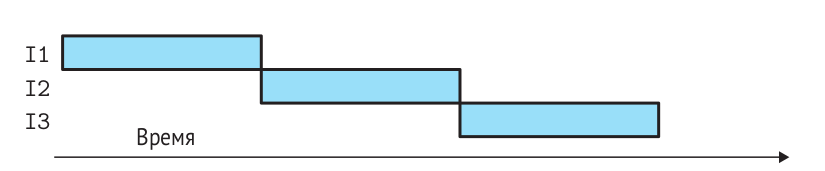
\includegraphics[width=1\linewidth]{scalar_example.png}
        \caption{Неконвейерная реализация}
    \end{minipage}\hfill
    \begin{minipage}{0.48\textwidth}
        \centering
        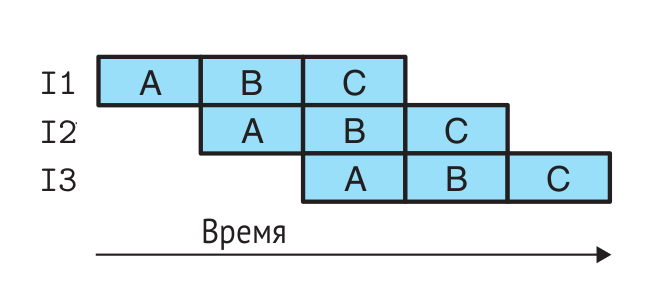
\includegraphics[width=1\linewidth]{parallel_example.png}
        \caption{Конвейерная реализация}
    \end{minipage}
\end{figure}

\textit{SIMD} (англ. single instruction, multiple data — одиночный поток команд, множественный поток данных) — принцип компьютерных вычислений, позволяющий обеспечить параллелизм на уровне данных.

Короткие SIMD инструкции (64 или 128 бит) стали появляться в 1990-х годах.
В 2010 году компания Intel представила SIMD-расширение AVX в процессорах архитектуры Sandy Bridge.

\textit{Intrinsic (англ. внутренний) функции} -  это функции, реализация которой специально обрабатывается компилятором. Как правило, она может заменять последовательность автоматически генерируемых инструкций для вызова оригинальной функции, подобно \textit{inline} функции. В отличие от \textit{inline} функции, компилятор обладает глубокими знаниями о \textit{intrinsic} функции и поэтому может лучше интегрировать и оптимизировать ее для конкретной ситуации.

\textit{Intrinsic} функции часто используются для векторизации и параллелизации. Компиляторы для C и C++ преобразуют \textit{intinsic} непосредственно в \textit{SIMD} инструкции.

\subsection*{Множество Мандельброта}
\begin{figure}[h]
    \centering
    
\includegraphics[width=1\linewidth]{mandelbrot_example.png}
    \caption{Пример визуализации множества Мандельброта}
\end{figure}
\textit{Множество Мандельброта} — множество точек c на комплексной плоскости, которое задается рекуррентным соотношением $Z_n = Z_n^2 + c$, где $Z_0 = 0$.

Иначе говоря, это множество таких $с$, для которых существует такое действительное $R$, что неравенство $|z_n| < R$ выполняется при всех натуральных n.\\

Множество Мандельброта является одним из самых известных фракталов, в том числе за пределами математики, благодаря своим цветным визуализациям
\subsubsection*{Построение множества}
Переформулируем соотношение, описанное выше. Заменим $Z_n$ на $x_n$ и $y_n$ и получим значения координат комплексной плоскости $(x, y)$:
\begin{align} 
    x_{n+1} = x_n^2 - y_n^2 + x_0 \nonumber\\
    y_{n+1} = 2x_ny_n + y_0 \label{calc_expressions}
\end{align}

Очевидно, что как только модуль $Z_n$ окажется больше 2, все последующие модули последовательности станут стремиться к бесконечности. В случае $|c| > 2$ это можно доказать с помощью метода математической индукции. При |c| > 2 точка c заведомо не принадлежит множеству Мандельброта, что можно вывести методом математической индукции, используя равенство $Z_0 = 0$.
\newpage

\section*{Виды реализаций вычислений множества Мандельброта}
\subsubsection*{Примитивный}
В данной реализации выражения (\ref{calc_expressions}) просто переведены в код на C, каждый пиксель обрабатывается отдельно

\begin{lstlisting}
    FOR EACH pixel on the screen (x0, y0)
        x := x0
        y := y0
    
        i := 0
        FOR i TO MAX_ITERATION_NUMBER
            IF x*x + y*y > 4 THEN
                BREAK
            END IF
    
            x = x*x - y*y + x0
            y = 2*x*y + y0
            i++
        ENDLOOP
        
        PAINT(x0, y0, i)
\end{lstlisting}
\subsubsection*{С векторизацией}
В данной реализации используются AVX2 инструкции, одновременной обрабатываются 8 пикселей.

\begin{lstlisting}
    FOR EACH 8 pixels on the screen (x0, y0)
        x := x0
        y := y0
        i := _mm256_setzero_si256();
        FOR i TO MAX_ITERATION_NUMBER
            x2      := _mm256_mul_ps(x,  x)
            y2      := _mm256_mul_ps(y,  y)
            xy      := _mm256_mul_ps(x,  y)
            radius2 := _mm256_add_ps(x2, y2)
    
            cmp_mask := _mm256_cmp_ps(radius2, MAX_RADIUS_2_256,
                                      _CMP_LT_OQ)
            IF (_mm256_testz_ps(cmp_mask, cmp_mask)) THEN
                BREAK
            END IF
    
            x = _mm256_add_ps(x0, _mm256_sub_ps(x2, y2))
            y = _mm256_add_ps(y0, _mm256_add_ps(xy, xy))
    
            iterations = _mm256_sub_epi32(iterations,
                         _mm256_castps_si256(cmp_mask))
        ENDLOOP
    
        PAINT(x0,y0, i)
\end{lstlisting}
Формально алгоритм остался таким же, но вместо чисел вектора из 8 чисел.

\section*{Экспериментальная установка}
Характеристики системы, на которой снимались значения:
\begin{table}[h]
    \centering
    \begin{tabular}{|c|c|}
        \hline
        OS         & Linux Mint 21.3 x86\_64 \\\hline
        Kernel     & 6.1.0-1036-oem          \\\hline
        CPU        & AMD Ryzen 7 5700U       \\\hline
    \end{tabular}
\end{table}


\section*{Методика измерений}
\begin{table}[h]
    \centering
    \begin{tabular}{|c|c|}
        \hline
        Разрешение           & 1600x900 \\\hline
        Количество вызовов   & 100      \\\hline
        Макс. Число итераций & 256      \\\hline
    \end{tabular}
    \caption{Параметры программы}
\end{table}
Количество тактов вычисляется с помощью функции clock() из библиотеки time.h.\\

Вычисляется разница тактов перед многократным вызовом функции и после.\\

Измерения проводятся для с флагами оптимизации -O0, -O1, -O2, -O3, -Os.\\

Влиянием температуры процессора, кэширования, пыли в компьютере, космических лучей мы пренебрегаем.

\section*{Результаты измерений}
\begin{table}[h]
    \centering
    \begin{tabular}{|l|l|l|l|l|l|}
    \hline
        ~ & -O0 & -O1 & -O2 & -O3 & -Os \\ \hline
        П* (такты) & 8934761 & 3249166 & 3309362 & 3310215 & 4047199 \\ \hline
        В* (такты) & 3233748 & 593930 & 601007 & 607176 & 628752 \\ \hline
        П* (такты / вызов) & 34901,41016 & 12692,05469 & 12927,19531 & 12930,52734 & 15809,37109 \\ \hline
        В* (такты/вызов) & 12631,82813 & 2320,039063 & 2347,683594 & 2371,78125 & 2456,0625 \\ \hline
        П* (кадры/с)  & 11,19224118 & 30,77712865 & 30,21730473 & 30,20951811 & 24,70844651 \\ \hline
        В* (кадры/с) & 30,92386915 & 168,3700099 & 166,3874131 & 164,6968918 & 159,0452197 \\ \hline
        П*/В* & 2,7629738 & 5,470621117 & 5,506361823 & 5,451821218 & 6,436876543 \\ \hline
        
    \end{tabular}
    \caption{Количество тактов для каждой конфигурации}
\end{table}
\centering П* - примитивный, В* - векторизированный

\end{document}
